\documentclass{amsart}

% --- PACKAGES ---
\usepackage[margin=1in]{geometry}
\usepackage{amsmath, amsthm, amssymb}
\usepackage[colorlinks=true, allcolors=black]{hyperref}
\usepackage{tikz} % For drawing diagrams

% --- DOCUMENT METADATA ---
\hypersetup{
    pdftitle={On the Evaluation of Certain Series at a Golden Ratio-Based Constant},
    pdfauthor={Tristen Harr},
    pdfsubject={Complex Analysis, Special Functions, Number Theory},
    pdfkeywords={Infinite Series, Polylogarithm, Golden Ratio, Special Functions, Numerical Analysis}
}

% --- THEOREM-LIKE ENVIRONMENTS (AMSART STYLE) ---
\theoremstyle{plain}
\newtheorem{theorem}{Theorem}[section]
\newtheorem{proposition}[theorem]{Proposition} % Corrected: Shares counter with theorem
\newtheorem{lemma}[theorem]{Lemma}
\newtheorem{corollary}[theorem]{Corollary}

\theoremstyle{definition}
\newtheorem{definition}[theorem]{Definition}
\newtheorem{conjecture}[theorem]{Conjecture}

\theoremstyle{remark}
\newtheorem*{remark}{Remark}

% --- CUSTOM OPERATORS AND COMMANDS ---
\newcommand{\LambdaG}{\Lambda_{G1}}

% ======================================================================
% --- BEGIN DOCUMENT ---
% ======================================================================

\begin{document}

\title[Series Evaluations at a Golden Ratio Constant]{On the Evaluation of Certain Series at a Golden Ratio-Based Constant}
\author{Tristen Harr}
\address{Saint Charles, Missouri, USA}
\email{tristen.harr@gmail.com}
\date{June 18, 2025}

\begin{abstract}
This paper introduces and analyzes a specific complex constant, denoted $\Lambda_{G1}$, which is uniquely derived from a set of defining principles related to the golden ratio, $\phi$. The motivation for this constant is shown to arise from a classical geometric construction. We first prove the constant's fundamental properties, including the convergence condition $|\LambdaG| < 1$. The primary contribution of this work is the systematic evaluation of two families of infinite series where $\LambdaG$ serves as the argument, connecting them to Eulerian polynomials and the Polylogarithm function, $\mathrm{Li}_s(\LambdaG)$. Furthermore, we present high-precision numerical evaluations for the Dilogarithm ($s=2$) and Trilogarithm ($s=3$) of this constant and, based on this evidence, we conjecture that these values are non-trivial transcendental numbers not expressible in terms of common mathematical constants.
\end{abstract}

\maketitle

% --- SECTION 1: INTRODUCTION ---
\section{Introduction}
The study of infinite series often reveals deep connections between different areas of mathematics. This paper focuses on the properties of series evaluated at a specific complex constant derived from the golden ratio, $\phi$. The motivation for this constant arises from the classical geometric problem of dividing a line segment in extreme and mean ratio. This problem provides a non-arbitrary foundation for a pair of "simplicity constraints" whose unique solution gives rise to the constant we analyze.

We define this constant, termed $\LambdaG$, and rigorously prove its properties. The purpose of this paper is to systematically explore the evaluation of several important families of infinite series using this constant as the primary argument. We will show that because $\LambdaG$ lies within the unit disk, it serves as a valid and interesting argument for well-known summation formulas. This work provides a careful cataloging of these results and culminates in a formal conjecture regarding the nature of the resulting values of the Polylogarithm function.

% --- SECTION 2: THE CONSTANT AND ITS PROPERTIES ---
\section{The Constant \texorpdfstring{$\Lambda_{G1}$}{Lambda\_G1} and its Foundational Properties}

\subsection{Defining Principles and Uniqueness}
We define two real constants, $T$ and $J$, as the unique solution to a pair of principles representing minimal structural simplicity, motivated by the geometric problem described in Appendix~A.

\begin{definition}[Defining Principles]
The constants $T$ and $J$ are the real numbers $(a,b)$ that satisfy:
\begin{enumerate}
    \item \textbf{Additive Simplicity:} $a+b = 1/2$.
    \item \textbf{Ratio Simplicity:} $a/b = \phi$, where $\phi = \frac{1+\sqrt{5}}{2}$.
\end{enumerate}
\end{definition}

\begin{theorem}[Uniqueness of the Constants]
The Defining Principles, subject to the convergence constraint $a^2+b^2 < 1$, admit a unique solution.
\end{theorem}
\begin{proof}
Substituting $a=b\phi$ into the first principle gives $b\phi+b=1/2$, which implies $b(\phi+1)=1/2$. Using the property $\phi+1=\phi^2$, we get $b\phi^2=1/2$, which yields the unique solution $b=(3-\sqrt{5})/4$. Subsequently, $a=\phi b = (\sqrt{5}-1)/4$. We define these unique constants as $T=a$ and $J=b$. The fulfillment of the convergence constraint is proven in Lemma~\ref{lem:convergence}.
\end{proof}

\begin{definition}[The Primary Constant]
The constant $\LambdaG$ is defined as the complex number $\LambdaG = T+iJ$.
\end{definition}

\subsection{Convergence Property}
A crucial property of $\LambdaG$ is that its magnitude is less than one, which guarantees the convergence of the power series we will investigate.

\begin{lemma}[Convergence of $\LambdaG$]
\label{lem:convergence}
The constant $\LambdaG$ lies within the unit disk, i.e., $|\LambdaG| < 1$.
\end{lemma}
\begin{proof}
Convergence requires $|\LambdaG|^2 < 1$. We calculate the squared values of the components:
$T^2 = \left(\frac{\sqrt{5}-1}{4}\right)^2 = \frac{6-2\sqrt{5}}{16}$ and $J^2 = \left(\frac{3-\sqrt{5}}{4}\right)^2 = \frac{14-6\sqrt{5}}{16}$.
Summing these gives:
\begin{align*}
    |\LambdaG|^2 &= T^2+J^2 = \frac{6-2\sqrt{5} + 14-6\sqrt{5}}{16} \\
                 &= \frac{20-8\sqrt{5}}{16} = \frac{5-2\sqrt{5}}{4} \approx 0.1309.
\end{align*}
Since $0.1309 < 1$, the condition is satisfied.
\end{proof}

% --- SECTION 3: POLYNOMIAL-WEIGHTED SERIES ---
\section{Evaluation of Polynomial-Weighted Series}
The first family of series we analyze are those weighted by polynomial powers of the index.

\begin{proposition}[Polynomial-Weighted Sums]
The infinite series $S_k = \sum_{n=0}^{\infty} n^k \cdot (\LambdaG)^n$, for any integer $k \ge 0$, converges to the value:
$$S_k = \frac{A_k(\LambdaG)}{(1-\LambdaG)^{k+1}}$$
where $A_k(x)$ is the k-th Eulerian polynomial.
\end{proposition}
\begin{proof}
The general formula for the sum of a polynomial-weighted geometric series is a known result in complex analysis (see, e.g., Abramowitz and Stegun \cite{AandS}). The formula is valid for any complex argument $x$ such that $|x|<1$. Since we have proven in Lemma~\ref{lem:convergence} that $|\LambdaG|<1$, the substitution of $\LambdaG$ into this formula is valid.
\end{proof}

% --- SECTION 4: RECIPROCAL-WEIGHTED SERIES ---
\section{Evaluation of Reciprocal-Weighted Series and the Polylogarithm}
The second family of series are those weighted by reciprocal powers of the index.

\begin{definition}[The Polylogarithm Function]
The Polylogarithm function of order $s$, $\mathrm{Li}_s(z)$, is defined by the power series:
$$ \mathrm{Li}_s(z) = \sum_{n=1}^{\infty} \frac{z^n}{n^s}. $$
This series converges for all complex numbers $z$ such that $|z|<1$.
\end{definition}

\begin{proposition}[Connection to the Polylogarithm Function]
The series $S_s = \sum_{n=1}^{\infty} \frac{(\LambdaG)^{n}}{n^s}$ converges for any complex $s$ to the value:
$$S_s = \mathrm{Li}_s(\LambdaG).$$
\end{proposition}
\begin{proof}
This result follows directly from the definition of the Polylogarithm function. Since we have proven $|\LambdaG| < 1$ in Lemma~\ref{lem:convergence}, the series is guaranteed to converge.
\end{proof}

% --- SECTION 5: NUMERICAL ANALYSIS AND CONJECTURE ---
\section{Numerical Analysis and a Conjecture on the Nature of \texorpdfstring{$\mathrm{Li}_s(\LambdaG)$}{Li\_s(Lambda\_G1)}}
We now investigate the nature of the specific values obtained in the previous section.

\subsection{Numerical Values}
We present high-precision numerical evaluations for the first two non-trivial integer cases of the Polylogarithm of $\LambdaG$, computed from the series definition.
\begin{itemize}
    \item For $s=2$, the Dilogarithm of $\LambdaG$ is:
    $$ \mathrm{Li}_2(\LambdaG) \approx 0.322328253720993 + 0.226730769307749i. $$
    \item For $s=3$, the Trilogarithm of $\LambdaG$ is:
    $$ \mathrm{Li}_3(\LambdaG) \approx 0.310345112613931 + 0.198884393433621i. $$
\end{itemize}

\subsection{A Conjecture on the Nature of These Values}
The numerical results above are presented as benchmark values for future research. Analysis using inverse symbolic calculators (such as the LLL algorithm) does not resolve these values into simple, closed-form expressions involving common mathematical constants. This leads us to propose the following.

\begin{conjecture}
For any integer $s \ge 2$, the value $\mathrm{Li}_s(\LambdaG)$ is a transcendental number that is not in the ring $\mathbb{Q}(\pi, e, \ln(2), \phi, \gamma)$.
\end{conjecture}
\begin{remark}
Proving this conjecture is beyond the scope of this paper, but proposing it frames a clear direction for future work and elevates the significance of the constant $\LambdaG$ as a tool for probing the structure of the Polylogarithm function.
\end{remark}

% --- SECTION 6: CONCLUSION ---
\section{Conclusion}
We have rigorously defined a complex constant, $\LambdaG$, derived from principles of simplicity related to the golden ratio and have proven its convergence. The primary contribution of this work is the systematic cataloging of the closed-form values for two important families of infinite series evaluated at this constant: those related to Eulerian polynomials and those defined by the Polylogarithm function $\mathrm{Li}_s(\LambdaG)$.

We have extended this analysis by providing high-precision numerical values for $\mathrm{Li}_2(\LambdaG)$ and $\mathrm{Li}_3(\LambdaG)$, and on this basis, have conjectured that these values are non-trivial transcendental numbers. This paper thus provides a complete, self-contained exploration, a set of benchmark results, and a new open problem related to this elegant mathematical constant.

% --- APPENDIX ---
\appendix
\section{Geometric Motivation for the Defining Principles}
\label{app:A}
The principles of simplicity presented in Section~2 are motivated by a classical compass-and-straightedge construction. Specifically, they represent the algebraic solution to the problem of dividing a line segment of length $1/2$ into two smaller segments, $T$ and $J$, such that their ratio is the golden ratio, i.e., $T/J = \phi$. This geometric origin provides a foundational, non-arbitrary basis for the algebraic framework.

\begin{figure}[htbp]
    \centering
    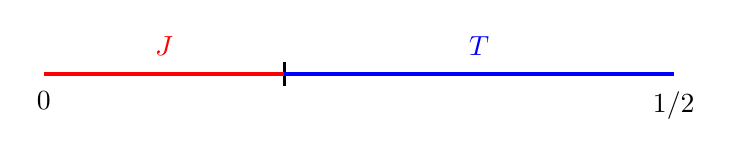
\begin{tikzpicture}[scale=1]
        % Robustly calculate lengths using \pgfmathsetmacro
        \pgfmathsetmacro{\phiVal}{(1+sqrt(5))/2}
        \pgfmathsetmacro{\totalLen}{8} % Visual length for the 1/2 segment
        \pgfmathsetmacro{\Tlen}{\totalLen / \phiVal}
        \pgfmathsetmacro{\Jlen}{\totalLen - \Tlen}
        
        % Draw the main line
        \draw[thick] (0,0) -- (\totalLen,0);
        
        % Add endpoint labels
        \node[below=3pt] at (0,0) {$0$};
        \node[below=3pt] at (\totalLen,0) {$1/2$};

        % Add a tick mark for the division
        \draw[thick] (\Jlen, -0.15) -- (\Jlen, 0.15);
        
        % Add labels for J and T (Corrected order from diagram)
        \node[above=3pt, red] at (\Jlen/2, 0) {$J$};
        \node[above=3pt, blue] at (\Jlen + \Tlen/2, 0) {$T$};
        
        % Color the segments
        \draw[line width=1.5pt, red] (0,0) -- (\Jlen, 0);
        \draw[line width=1.5pt, blue] (\Jlen,0) -- (\totalLen,0);
    \end{tikzpicture}
    \caption{A visual representation of the geometric problem giving rise to the constants T and J.}
    \label{fig:geometry}
\end{figure}

% --- BIBLIOGRAPHY ---
\begin{thebibliography}{9}

\bibitem{AandS}
M. Abramowitz and I. A. Stegun (eds.), \textit{Handbook of Mathematical Functions with Formulas, Graphs, and Mathematical Tables}, 10th printing, with corrections, Dover, New York, 1972.

\end{thebibliography}

\end{document}